\documentclass{article}
\usepackage{graphicx}
\usepackage{wrapfig}
\usepackage{subcaption}
\usepackage[margin=1in]{geometry}
\usepackage{amsmath} % or simply amstext
\usepackage{siunitx}
\usepackage{booktabs}
\usepackage[export]{adjustbox}
\newcommand{\angstrom}{\textup{\AA}}
\usepackage{cleveref}
\usepackage{booktabs}
\usepackage{gensymb}
\usepackage{float}

\title{Supplmental Information : Understanding the nanoscale structure of hexagonal phase lyotropic liquid crystal membranes}
\author{Benjamin J. Coscia \and Douglas L. Gin \and Richard D. Noble \and Joe Yelk \and Matthew Glaser \and Xunda Feng \and Michael R. Shirts}

\begin{document}

\graphicspath{{./figures/}}  % put all the figures here
\maketitle

n{itemize}
                %MRS2: make clear sampling what?
                \item We are interested in 5 pore-to-pore distances which should all be equal in
                a perfect hexagonal array, however only 4 distances are independent % can visualize this in supplemental material. Will make a lot of things more clear below.
                \item Each pore spacing has its own trajectory of spacing vs. time. Using data collected after
                the system is equilibrated, we calculate how long it takes for the data in each of the 5
                trajetories to become uncorrelated using pymbar.timeseries.integratedAutocorrelationTime() % reference
                \item We break the full trajectories down into sub-trajectories based on the
                maximum autocorrelation time of those found in the previous step.
                \item For each bootstrap trial, we recreate an equilibrium trajectory by randomly
                sampling pore spacings from the sub-trajectories
                \item We get an average value for each pore spacing by finding the mean of the bootstrapped data
                \item We calculate the overall average as the mean of all bootstrapped pore spacings
                  %MRS3: this sounds a little convoluted below.  Should just be the standard error in the boostrap estimates of the pore spacing?
                  %MRS3: this can be fixed in the draft not outline.
                \item The uncertainty for each pore spacing is calculated as $\dfrac{<x> - x}{4}$ where $<x>$ is the
                average spacing from the bootstrap trial and $x$ is the average value of one of the pore spacings.
                \item We report the mean of these uncertainties
                % MRS: need to deal with the fact only 4 are independent in the bootstrapping?  How did we do that?
                % BJC: Updated
        \end{itemize}

\begin{wrapfigure}{R}{0.4\textwidth}
      \centering
      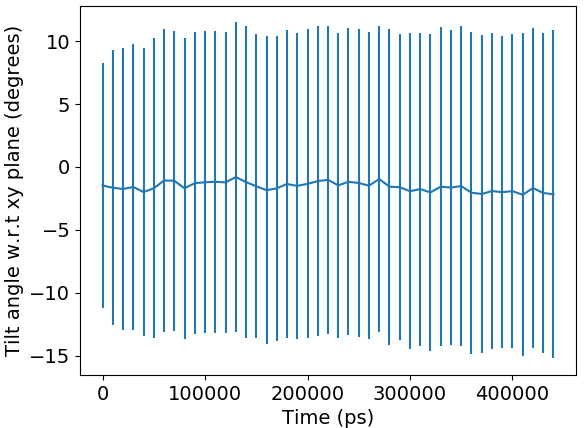
\includegraphics[width=0.4\textwidth]{tilt.png}
      \caption{The average angle between alkane chains and the xy plane is nearly zero degrees}\label{fig:tilt}     
\end{wrapfigure}


\begin{figure}
	\centering
	\begin{subfigure}{0.45\textwidth}
		\centering
		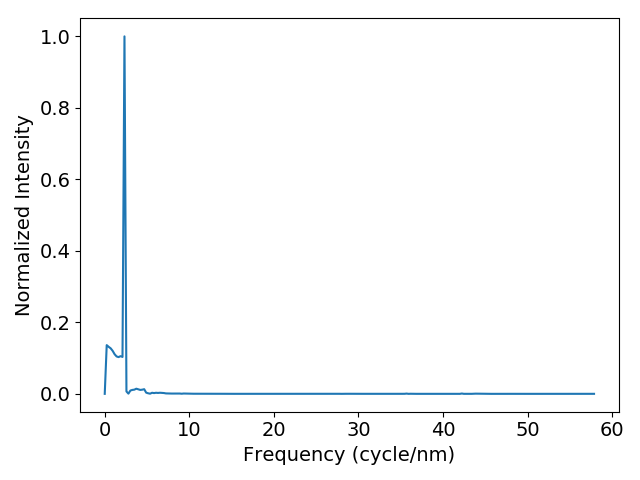
\includegraphics[width=\textwidth]{ps5layered.png}
		\caption{}\label(fig:ps5layered}
	\end{subfigure}
	\begin{subfigure}
		\centering
		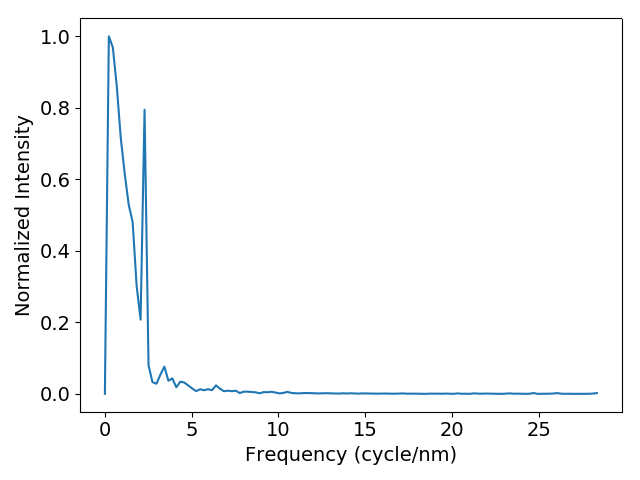
\includegraphics[width=\textwidth]{ps5offset.png}
		\caption{}\label{fig:ps5offset}
	\end{subfigure}
\end{figure}


\begin{figure}[!ht]
        \centering
        \begin{subfigure}{0.45\textwidth}
                \centering
                \hspace{-1cm}
                \vspace{1cm}
                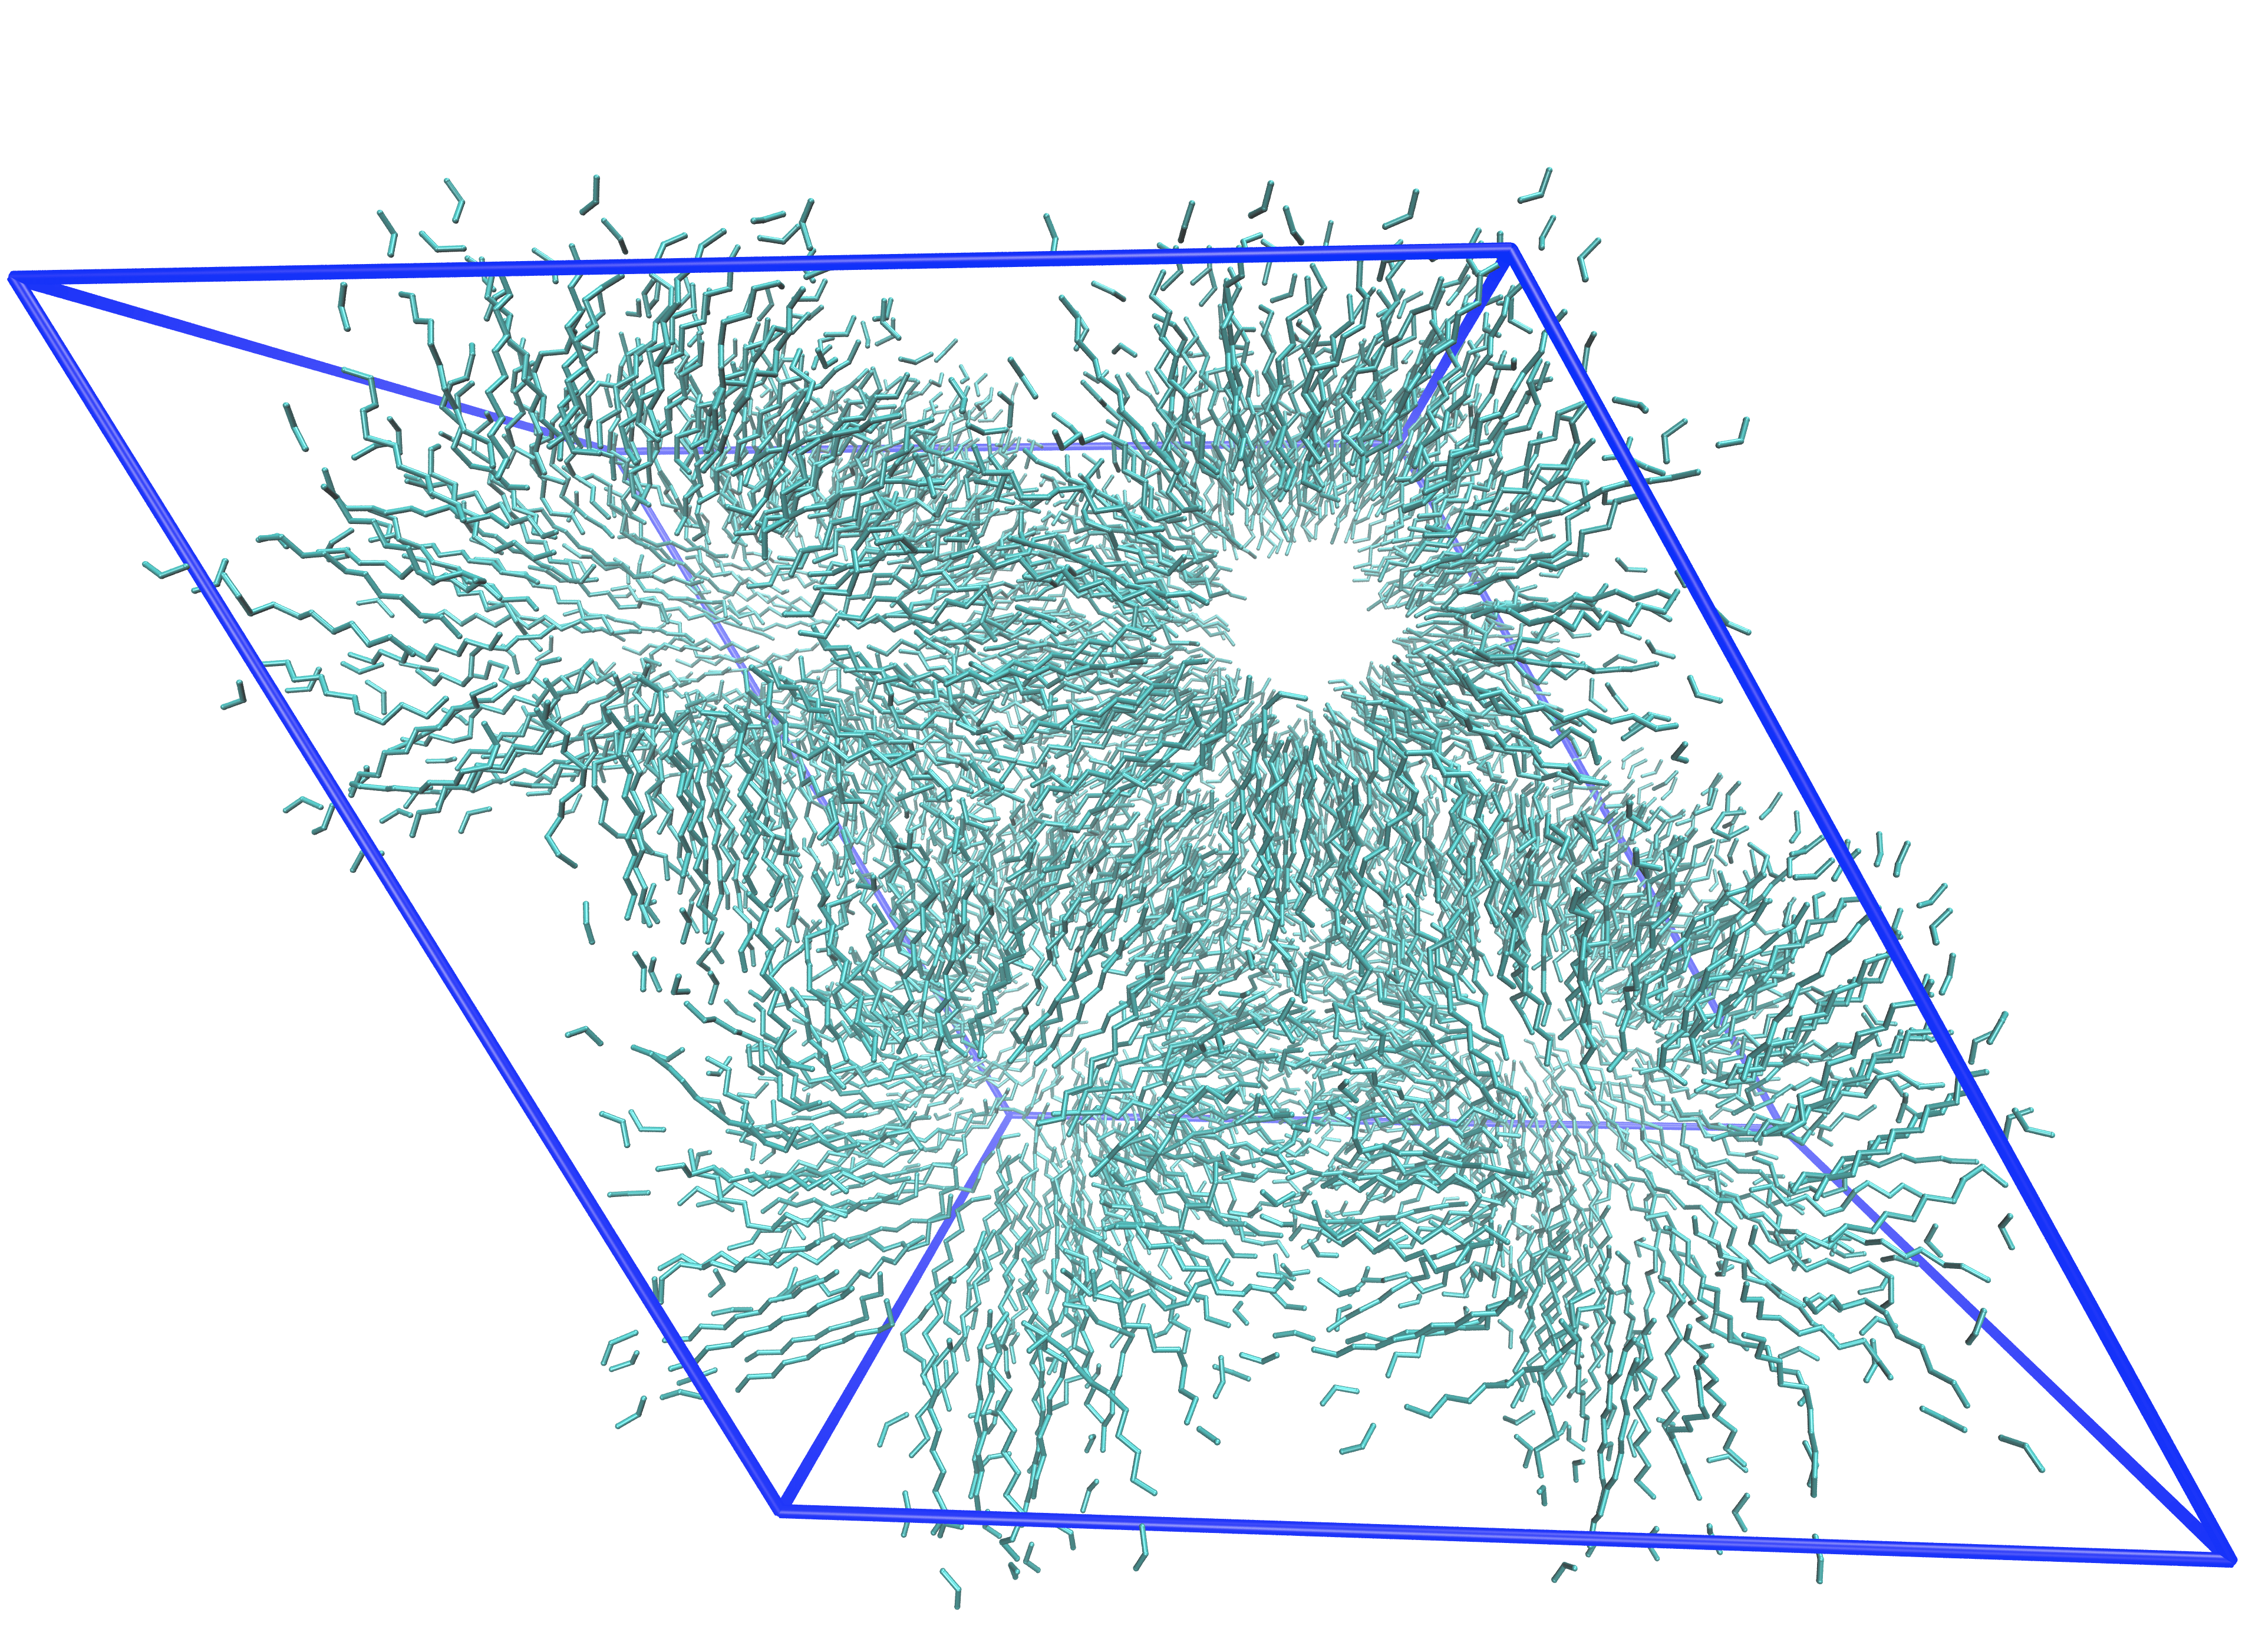
\includegraphics[width=\textwidth,scale=2]{tails_topview.png}
                \caption{}\label{fig:tails_topview}
        \end{subfigure}
        \begin{subfigure}{0.45\textwidth}
                \centering
                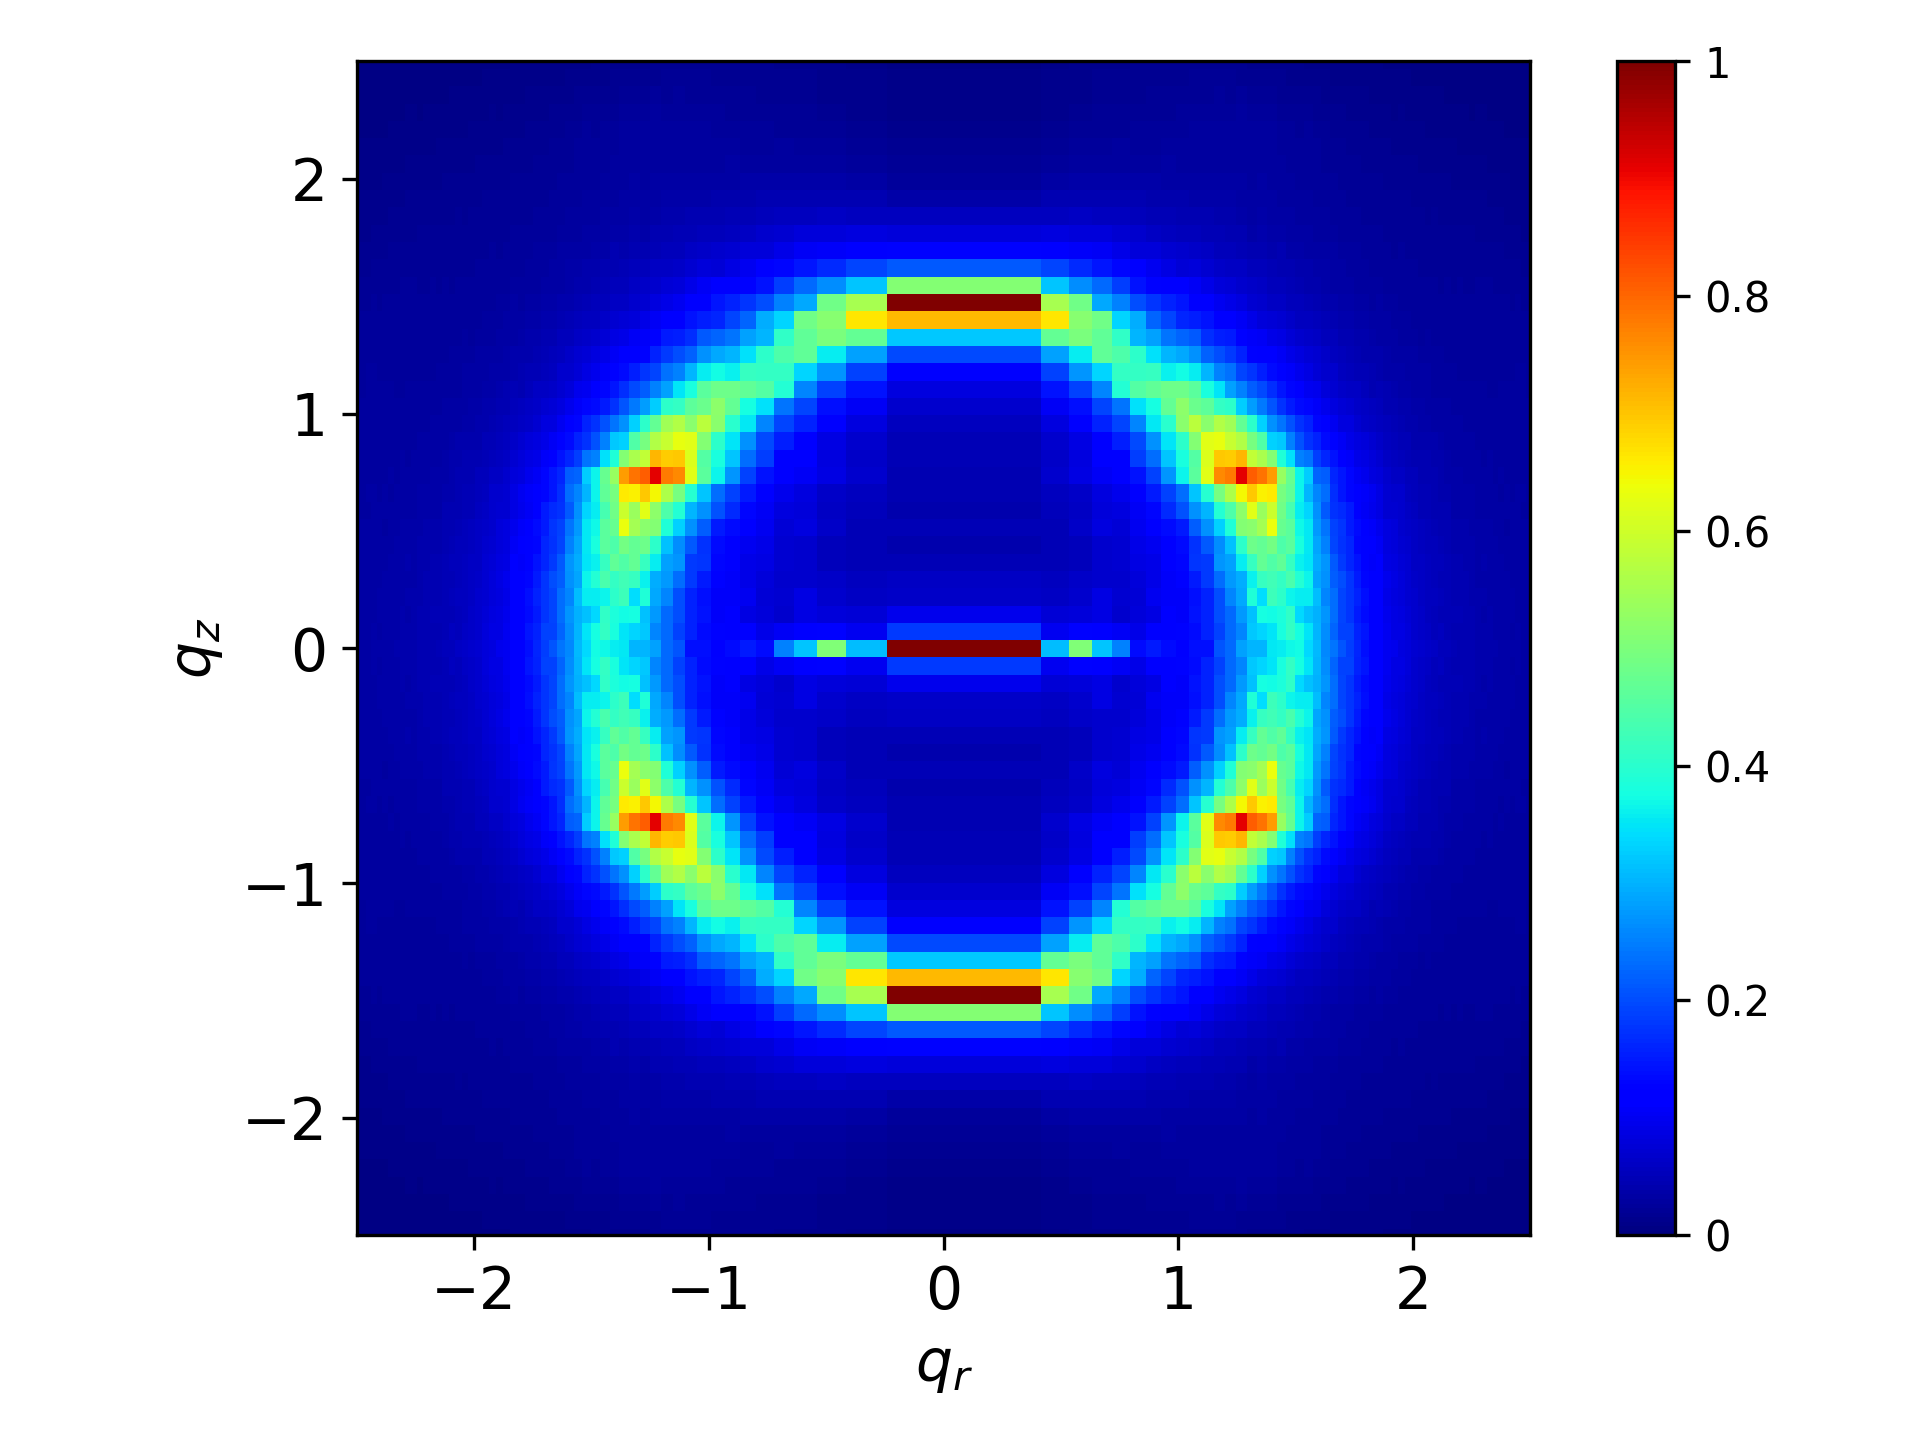
\includegraphics[width=\textwidth]{tails_rzplot.png}
                \caption{}\label{fig:tails_rzplot}
        \end{subfigure}
        \begin{subfigure}{0.45\textwidth}
                \centering
                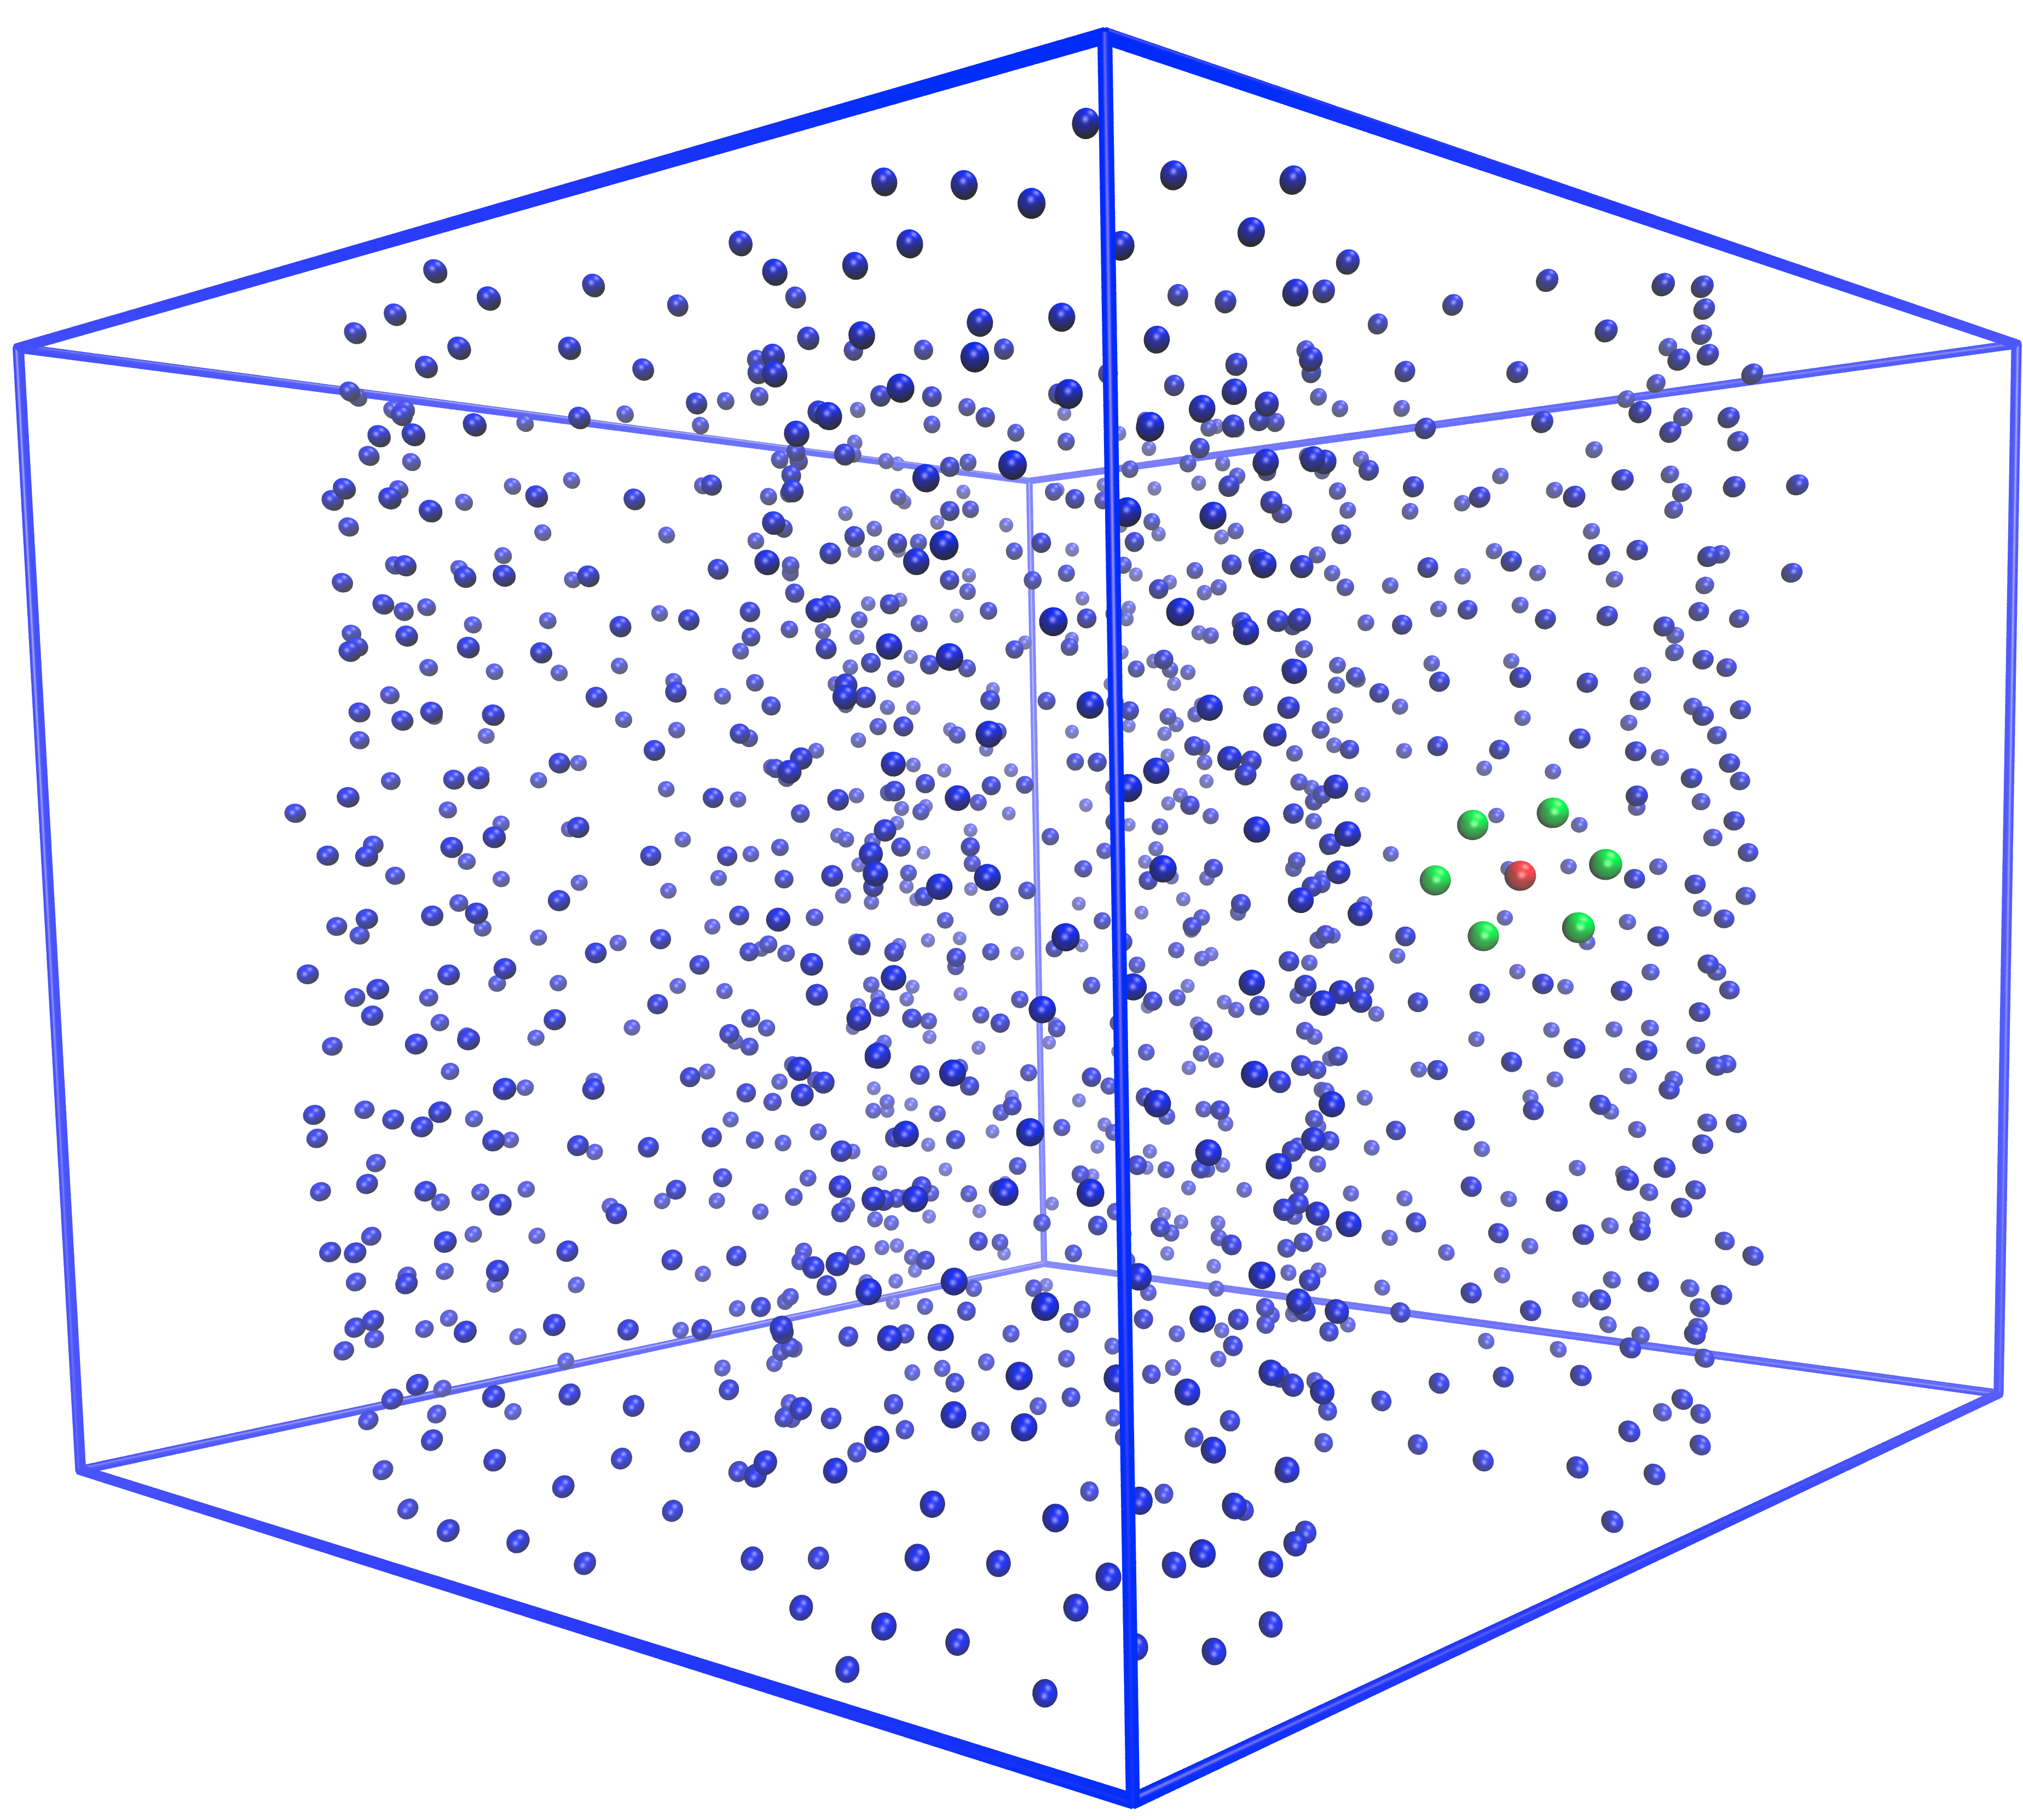
\includegraphics[width=\textwidth]{centroids_box.png}
                \caption{}\label{fig:centroids}
        \end{subfigure}
        \begin{subfigure}{0.45\textwidth}
                \centering
                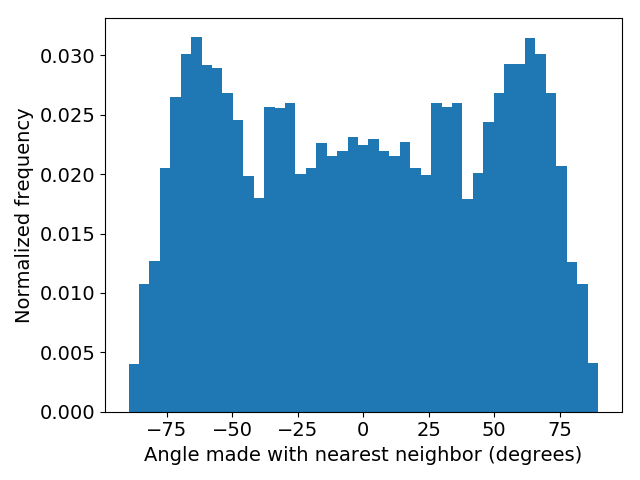
\includegraphics[width=\textwidth]{angles_traj_layered.png}
                \caption{}\label{fig:angle_distribution}
        \end{subfigure}
        \caption{(a) The trajectory can be stripped of all atoms except carbon
        atoms in monomer tails. (b) Simulated diffraction of the tail-only trajectory
        still gives rise to R-spots. (c) Finding the center of mass and visualizing
        their coordinates reveals the hexagonal-like packing of the tails. (d) The
        distribution created by measuring the angle between each centroid (e.g. red
        in (c)) and its neareset neighbors (e.g. green in (c)) with respect to the xy
        plane has distinct spikes near 30\degree, which is consistent with the location
        of R-spots}\label{fig:tail_packing}
\end{figure}



\end{document}
